% UG project example file, February 2024
%
%   Added the "online" option for equal margins, February 2024 [Hiroshi Shimodaira, Iain Murray]
%   A minor change in citation, September 2023 [Hiroshi Shimodaira]
%
% Do not change the first two lines of code, except you may delete "logo," if causing problems.
% Understand any problems and seek approval before assuming it's ok to remove ugcheck.
\documentclass[logo,bsc,singlespacing,parskip,online]{infthesis}
\usepackage{ugcheck}


% Include any packages you need below, but don't include any that change the page
% layout or style of the dissertation. By including the ugcheck package above,
% you should catch most accidental changes of page layout though.

\usepackage{etoolbox}
\usepackage[nopatch=footnote]{microtype} % recommended, but you can remove if it causes problems
%\usepackage[round]{natbib} % recommended for citations
\usepackage[natbib=true,style=numeric]{biblatex}
\addbibresource{refs.bib}
\usepackage{graphicx}
\usepackage{xcolor}
\usepackage{hyperref}
\usepackage{doi}
\usepackage[nameinlink]{cleveref}
\crefname{todo}{TODO}{TODOs}
\usepackage{todo}
\usepackage{comment}

\begin{document}
\begin{preliminary}

\title{Extensions to libseff, an effect handler implementation using continuations in C}

\author{Jamie Day}

% CHOOSE YOUR DEGREE a):
% please leave just one of the following un-commented
%\course{Artificial Intelligence}
%\course{Artificial Intelligence and Computer Science}
%\course{Artificial Intelligence and Mathematics}
%\course{Artificial Intelligence and Software Engineering}
%\course{Cognitive Science}
%\course{Computer Science}
%\course{Computer Science and Management Science}
%\course{Computer Science and Mathematics}
%\course{Computer Science and Physics}
%\course{Software Engineering}
\course{Master of Informatics} % MInf students

% CHOOSE YOUR DEGREE b):
% please leave just one of the following un-commented
\project{MInf Project (Part 1) Report}  % 4th year MInf students
%\project{MInf Project (Part 2) Report}  % 5th year MInf students
%\project{4th Year Project Report}        % all other UG4 students


\date{\today}

\abstract{
Effect handlers are a control flow paradigm that allow functions to perform \textit{effects}, which return control to a previously defined \textit{handler} for that effect, which may then perform arbitrary tasks and pass around the \textit{continuation} of the suspended function, which may then be resumed with some data, or terminated. The \textit{resolution} of which handler should handle a given effect call is a vital part of the design of such systems. \textbf{libseff} is a library for C that implements effect handlers using coroutines, in an efficient and programmer-friendly manner. This dissertation details the implementation and evaluation of a more expressive system for effect identification and resolution. Issues that would have made the adoption of libseff for large codebases highly impractical have been resolved, and although the new implementation runs slower than the old implementation in cases where handler resolution takes up a significant portion of runtime, these cases are shown to be rare in practice, and hence the extra expressiveness comes with no significant performance impact.
}

\maketitle

\newenvironment{ethics}
   {\begin{frontenv}{Research Ethics Approval}{\LARGE}}
   {\end{frontenv}\newpage}

\begin{ethics}

This project was planned in accordance with the Informatics Research
Ethics policy. It did not involve any aspects that required approval
from the Informatics Research Ethics committee.

\standarddeclaration
\end{ethics}


\begin{acknowledgements}
%I would like to thank Saj's Shawarma and Grill, for always having my back through these hard times.
I would like to thank my parents, Simon and Gill, for their unwavering support throughout this process, and my supervisor Sam for your patience. 
\end{acknowledgements}


\tableofcontents
\end{preliminary}


\chapter{Introduction}

\section{Handlers' History and Usage}
Effect handlers are a control-flow paradigm that have been growing in popularity recently. \citep{effekt-paper} First invented as a programming construct at the University of Edinburgh, they have come into use by companies worldwide, including GitHub and Uber, and are used by tens of millions of developers worldwide through React's Hook implementation. \citep{impact_study}

While the first description of effect handlers in \citet{og-paper} was written in "a style that required
considerable mathematical sophistication to understand", \citep{impact_study} a later position paper by \citeauthor{action-position-paper} served to popularise the abstraction.

\section{What even are effect handlers?}
An \textit{effect} is an operation or group of operations that can be \textit{performed} to do some kind of action that cannot be done from local code. 

Effect handlers can be conceptualised in many ways. One way of thinking about effect handlers, and the lens through which the abstraction was originally invented in \cite{og-paper}, is as a generalisation of exception handlers - an exception handler that can return to the point the exception was raised is an effect handler. \citep{ocaml-paper}

Effect handlers can also be considered as calls to a function whose implementation depends on context, and which is not guaranteed to return. Which handler will handle the effect (and hence in this interpretation implement the function) depends on the context in which this block of code is running. \citep{award-paper}

\section{What is libseff?}

\textbf{libseff} is an implementation of this idea in C. Differentiating \textbf{libseff} from other implementations of effect handlers in C is its intended use by the general programming community, rather than specifically compiler writers, as is the case with languages such as \textbf{libmpeff}. \citep{libseff_paper} \citep{libmprompt} \textbf{libseff} is also designed to be as lightweight as possible to allow its use in embedded systems. \citep{libseff_paper}

\textbf{libseff} at the time of writing has several peculiarities that make it unsuitable for use in production code in a large codebase. For example, the following code defines an effect: 
\begin{figure}[ht]
    \centering
    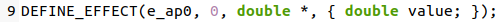
\includegraphics[width=0.9\linewidth]{eff_def.png}
    \caption{Taken from the ad.c test in the \textbf{libseff} repo}
\end{figure}

The leftmost argument to the macro is the name of the effect. The next argument is the ID of the effect, and this will be discussed below. The final arguments are the return value of the effect and a struct representing the parameters to the effect (all effects in \textbf{libseff}, barring the return effect, must return a struct).

The ID is an integer that is used for the representation of effects - the PERFORM macro passes this value to the handler resolution function to find the relevant handler, for example. Requiring this to be predefined by the programmer is quite unusual and inconvenient - more on this in \Cref{method}.

Another issue relating to the implementation of \textbf{libseff} is that only a maximum of 64 effects can be defined - again, more on this in \Cref{method}.

\section{This Project}

The aim of this project was to address the above limitations and extend libseff to allow the definition of (for all intents and purposes) an unlimited number of effects, and to remove the need to supply a manual, unique effect tag upon definition.

In \Cref{background}, this dissertation discusses the history of effect handlers, the many subtle differences in how this abstraction can be implemented, and the pros and cons of each. This section will provide the context for the development of \textbf{libseff} and why it was created, as well as some of the specifics about how it works.

\Cref{method} covers the parts of \textbf{libseff} that inspired this project, how they are potentially problematic, and the details of the solutions that have been implemented to fix these restrictions.

\Cref{eval} details the benchmarking and performance of these changes in the worst case and also more generally in normal code. Changes are suggested, implemented, checked and rebenchmarked that alleviate some of these issues. The implications of the impact on performance this causes for the median program  are evaluated.

Finally, in \Cref{conc}, this project and its implications are summarised and the potential for future work is discussed.





\chapter{Background} \label{background}

\section{What are effect handlers?}
Effect handlers are a control flow mechanism that can be considered in several different ways: for example, as a generalisation of exception handlers. \citep{sep-log} The only difference is that exception handlers cannot return to the site where the exception was raised - effect handlers can. More specifically, effect handlers are passed a continuation, (often restricted in some way, such as delimitation \citep{old-paper}), that represents the code that requested the effect.

Such abstractions have many potential applications, including for backtracking, cooperative multi-threading and more \citep{effect_handlers_tutorial}. Real-world usage of this abstraction is already a reality, with use by Uber, Google, Facebook and more. \citep{impact_study}

Effect handler semantic systems have three parts:
\begin{itemize}
\item An \textit{effect signature}, which defines an effect
\item The instantiation of a \textit{handler}, which will handle the passed in coroutine
\item The site where the effect is performed
\end{itemize}

In Effekt \citep{effekt-paper} these three things look like this:

\begin{figure}[ht]
    \centering
    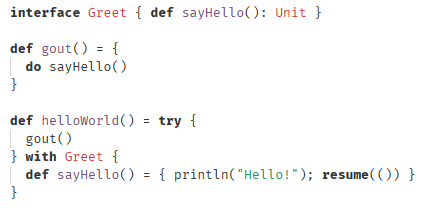
\includegraphics[width=0.5\linewidth]{basic_demo.png}
    \caption{Three parts of Effekt code showing the three different components of effect handlers. Adapted from \url{https://effekt-lang.org/quickstart}}
    \label{fig:basic}
\end{figure}

Let us expand from this basic example with something more involved:

\begin{figure}[ht]
    \centering
    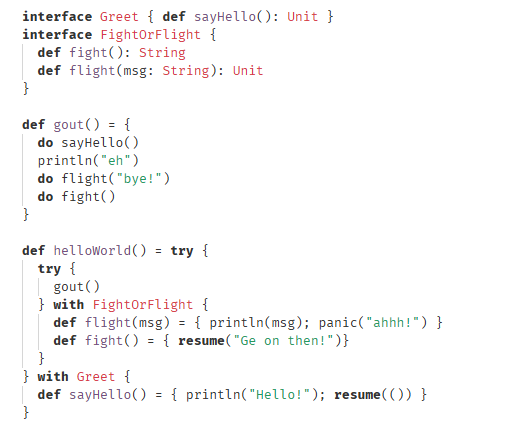
\includegraphics[width=0.9\linewidth]{effekt_2.png}
    \caption{More complex Effekt code}
    \label{fig:efkt2}
\end{figure}
\pagebreak
From this program we recieve the following output:

\begin{figure}[ht]
    \centering
    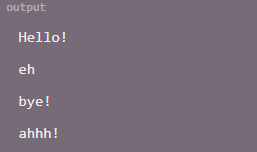
\includegraphics[width=0.5\linewidth]{effekt_2_out.png}
    \caption{Program output}
\end{figure}

This program displays several of the characteristic behaviours of effect handlers. First, note that effects will be handled in the closest (most recently wrapped) suitable handler - but that is not necessarily the closest handler. Further, the \textcolor{purple}{flight} operation is not required to return to the calling function; it is at the handler's discretion. Note also that data can be passed in and out of operation performances.


\section{Variants}
There are several different interpretations and implementations of effect handlers, with varying degrees of expressiveness and intuitiveness. Below are some of the more relevant divides.

\subsection{Lexical vs Dynamic binding and the Handler Stack}

When an effect of a specific type is performed, which handler should the program execute? 

Two methods for binding/scoping/resolving handlers are lexical and dynamic binding. These differ by what happens when an effect is called by code - dynamically bound handlers must traverse a call stack to find the closest handler for that effect, whereas lexical handlers (at least in theory) can get around this restriction.

Lexical binding has the advantage that handler resolution is a constant-time operation, but requires either a restrictive implementation or an expansive type system. As C barely possesses a type system at all, it was logical that \textbf{libseff} would use dynamic binding.

\subsection{Grouped vs Ungrouped Operations}

While in the ungrouped form effects are a single operation that is performed by itself, and a handler can handle many effects, with grouped operations an effect is a group of operations, and each handler can only handle one group. In this way effect definition looks more like interface definition in Java for example. \textbf{libseff} uses ungrouped effects (sometimes called singleton effects \citep{effekt-website}), which could be considered to be to be more useful for the average programmer than the libmpeff implementation, which is grouped.

\subsection{Single vs Multishot continuations}

A handler that uses singleshot continuations can only resume a given continuation once, after which it will be overwritten by a new continuation or in some other way made invalid. Multishot continuations allow a given continuation to be resumed more than once, which has applications in tasks including tree searches, back-tracking, and non-deterministic algorithms. Since a given coroutine must be able to run more than once in such systems, coroutines cannot run in place and the coroutine's portion of the stack must be copied. Since stack copying is unsafe in C given the possibility of escaping pointers into the stack, stack copying is unfeasible for most libraries that call user-provided functions, and hence \textbf{libseff} has single-shot continuations.

\subsection{Shallow vs Deep effect handlers}

A shallow effect handler binds an unhandled continuation when called, whereas a deep handler retains its binding over the continuation for subsequent calls. This is equivalent to saying that resumptions from a shallow handler do not return to that handler, whereas for deep handlers once a continuation has been wrapped in a handler it is always so. All shallow handlers can be turned into deep handlers by applying them recursively to continuations, although this can complicate type systems and be hard to reason about formally. \textbf{libseff} uses a combination of shallow and deep handlers, referred to as \textit{sheep} handlers after the name was coined in \textcite{wasmFX}
This means that the original handler is not automatically installed when continuation resumes, although there must be some handler installed. In \textbf{libseff} specifically, the effect set may be empty. \citep{libseff_paper}



\section{What is libseff?}

Although much of the current usage of effect handlers is found in functional languages, there exist libraries that implement effect handling in almost every major language in which it is possible, including C. However, these libraries, namely \textbf{libmpeff} and \textbf{libhandler}, are mostly designed specifically for compiler implementation, and as such offer features and make implementation decisions that do not necessarily make sense for the generic use case.\citep{libmprompt} \textbf{libseff}, on the other hand, is an implementation of effect handlers for C that is designed to be used directly by programmers.\citep{libseff_paper}








\chapter{Methodology} \label{method}

\section{ID assignment}

Before effects can be used in \textbf{libseff}, their types and ID must first be defined, in something similar to a function signature. Below we find the "effect signature" of an effect in \textbf{libseff}:

\begin{figure}[ht]
    \centering
    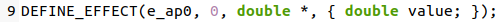
\includegraphics[width=0.9\linewidth]{eff_def.png}
    \caption{Taken from the ad.c test in the libseff repo}
\end{figure}

The leftmost argument to the macro is the name of the effect. The next argument is the ID of the effect, and this will be discussed below. The final arguments are the return value of the effect and a collection of the parameters to the effect, if any. In this way effects can have the same type-checking as provided by a normal C function.

Note that the ID is an integer. This value must be provided by the programmer at compile time, and it must be unique across all used files - and it is the programmer's job to ensure this. This would be time-consuming to maintain by hand in large codebases and is also unnecessarily dangerous, as \textbf{libseff} does not inform the programmer if their ID is not unique.

This causes particular difficulties when external libraries that also use effects are considered:  the requirement of unique tag selection across translation units "limits expressiveness ... [and] introduces the potential for insidious bugs when different libraries introduce distinct operations that share the same tag."\cite{libseff_paper} Since \textbf{libseff} uses dynamic binding\cite{libseff_paper}, the handler stack\todo* must be traversed to find the nearest handler for the given effect. If effects are intermingled between libraries, as shown below\todo{insert two images, one with the definitions of these functions and another with the handler stack}, then an effect performed by one coroutine can be erroneously intercepted by an enclosing handler from another library, with entirely unpredictable consequences, given the two effects need not even have the same type!

Therefore, a goal of this project was to have some method for automatically assigning IDs, with the following requirements:

\begin{itemize}
\item IDs must be unique within and between linked translation units
\item The number of IDs able to be defined must not be significantly constrained
\item Given the above constraints, checking whether a handler handles a given effect should be as fast as possible
\end{itemize}

One method for GUID generation that meets the above requirements is to use the address of allocated memory as IDs. Since pointers to different objects are guaranteed to be unequal in C\textcite[see § 6.5.10 para 7]{iso9899-2024}, simply ensuring the address isn't deallocated will mean that IDs generated in this fashion are unique. This trick is also used in the \textbf{libmprompt} library, see \href{https://github.com/koka-lang/libmprompt/blob/main/include/mpeff.h#L155}{here}.\cite{libmprompt}

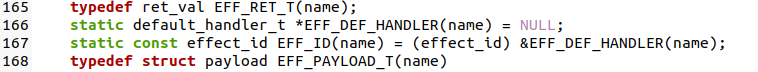
\includegraphics[scale=0.7]{ID_def_code.png}

Since tags are really just pointers to somewhere in memory, we may as well use this to store some information about the effect at this address - for static effects, this points to a global variable that holds a pointer that points to the set default handler implementation, i.e. \todo{image of typedef of effect id} $*eff\_id = some\_default\_handler\_location$. This stands as opposed to the prior representation, of an array of preset size holding pointers to default handlers, which is quite unusable when that size is the size of your entire memory.


This change in types and assignment time has carry-on effects on the rest of the library, including that switching on the effect ID returned by $seff\_resume$ is no longer possible, since the ID of a given effect is not a constant at compile time and hence cannot be used in \textcolor{teal}{case} statements. A new macro was introduced, $CASE\_SWITCH$, and the $CASE\_EFFECT$ macros redefined (see \cref{Syntax}), so that these are simply \textcolor{teal}{if} statements under the hood. This will be less performant for handlers that handle large numbers of effects, but that is expected to be relatively rare in actual code.

\section{Effect set representation}

\subsection{Prior implementation}

Previously, effect sets were represented as a 64-bit integer, with each index representing whether the effect with the ID at that index is handled, as below:

\begin{figure}[ht]
    \centering
    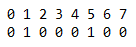
\includegraphics[width=0.3\linewidth]{effect_set.png}
    \caption{This 8-bit effect set handles effects 1 and 5, along with the return effect}
\end{figure}

This is a swift and lightweight implementation that is unfortunately quite unsuitable for use in environments with many defined effects, as the 64 effect limit is restrictive, and the naive solution of extending the indices available scales terribly - the memory per effect set is proportional to the number of effects! One of the primary goals of this project was to resolve this limitation.

\subsection{Current implementations} \label{impls_here}

Several other implementations have been created and benchmarked, and will be detailed below. Their relative performance is discussed in \Cref{eval}.

The first implementation created stored 

\begin{figure}[ht]
    \centering
    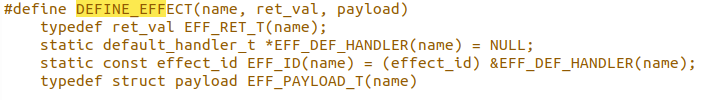
\includegraphics[width=1\linewidth]{defeff.png}
    \caption{Effect Definition}
    \label{fig:joooo}
\end{figure}

\section{Syntax changes} \label{Syntax}

These changes required changes to the syntax of the \textbf{libseff} library. Effect definition now does not require a manual tag to be provided, as was one of the goals of this project, but other common patterns in the usage of the \textbf{libseff} library, as shown through the many tests and benchmarks written for it, must also be 

Users now no longer have to (and can't) specify the ID of effects they define. More subtly, a common pattern seen even in the libseff code written to test and benchmark the library was for a handler to switch on the ID of an effect after being called - something no longer possible with effect IDs that aren't defined at compile time. These cases were rewritten as macros that inline to simply being if statements instead, which is less efficient for large switches but unlikely to come up in practise.

This syntax is slightly more unwieldy but ultimately the provided macros are simply syntactic sugar for unpacking the payload and do not need to be used for users to apply the full range of \textbf{libseff}. \todo{Cooler syntax, maybe side by side?}

\begin{figure}[ht]
    \centering
    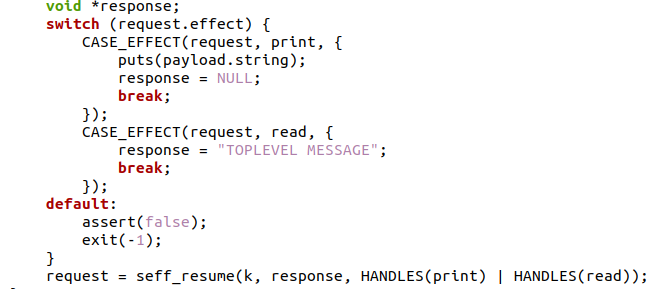
\includegraphics[width=1\linewidth]{oldswitch.png}
    \caption{The old switch implementation}
    \label{fig:oldswitch}
\end{figure}

\begin{figure}[ht]
    \centering
    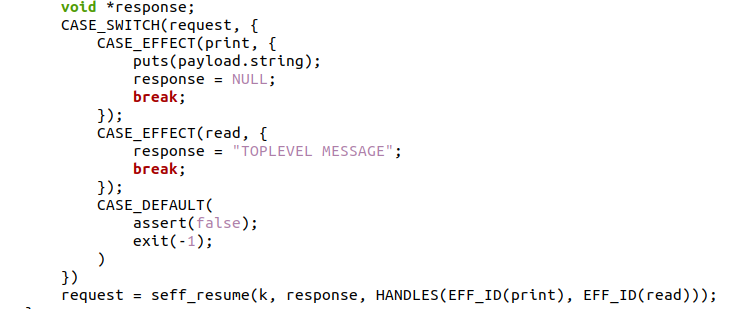
\includegraphics[width=1\linewidth]{newswitch.png}
    \caption{The new switch implementation with macros}
    \label{fig:newswitch}
\end{figure}

\section{Generative Effects}

In the new implementation, the dynamic generation of new effect IDs is possible, through provided functions $seff\_alloc\_gen\_id$ and $seff\_dealloc\_gen\_id$. These functions allocate and deallocate, respectively, a new node to a doubly linked list, where the address of nodes represents effect IDs. This guarantees the independence of these IDs from each other and from already allocated IDs for as long as the node remains allocated.

As normal effect tags can be considered to be double pointers to effect handlers, so too can generated tags: the first value of every node is a pointer to the location of the default handler, as shown below:\todo

One potential drawback of generative effects is that their effect IDs need to be manually passed around.\todo{do more research on generative effects} Another is that the programmer must take care to manually clean up generated effects when done with them, as is standard practice in C, and this may be more difficult than usual in an environment with unusual control flow, as coroutines tend to produce. This is already the case with the definition of \textit{coroutine} objects. Finally, generative effects do not provide any type-checking, and cannot use the base macros ($PERFORM$, $YIELD$, $THROW$) and must manually call the backend functions instead - automating this process and re-providing some type-checking is a possible area for future work.





\chapter{Evaluation} \label{eval}

The new implementations were tested against the existing tests for the \textbf{libseff} library, along with some new tests, such as a test of the new capability to provide generative effects and those effects' implementation of default handler capability (see \cref{appx} for details). All of these tests were passed; the new software is correct, and performs to the specification.

\begin{figure}[ht]
    \centering
    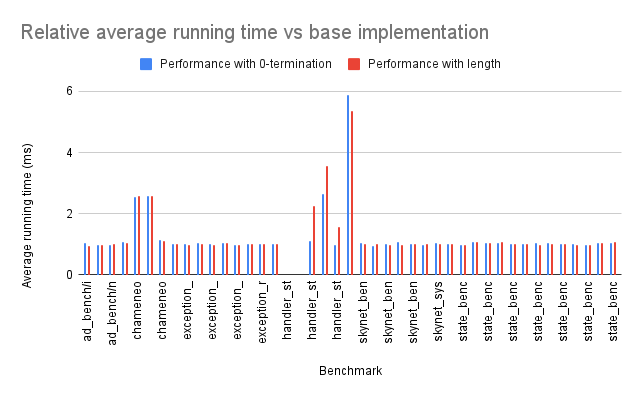
\includegraphics[width=1\linewidth]{all.png}
    \caption{Runtime of benchmarks as a proportion of original runtime}
    \label{fig:many}
\end{figure}

Benchmarks used by the original \textbf{libseff} library were rewritten to use the new syntax introduced (see \cref{method}), and in some cases the default number of iterations was adjusted: the $ad\_bench$ benchmark, for example, had to be increased to get results that were not mostly random noise, and the $exception\_bench$ family of benchmarks was revised down to allow for efficient benchmarking, as their runtimes were observed to remain consistent even with the decreased iteration counts. These benchmarks can be found in \cref{fig:many}.

These results show that in many normal programs using \textbf{libseff}, the performance implications of these changes are imperceptible, and cannot be discerned from random noise. The exception is in the benchmark specifically designed to test \textbf{libseff} in the worst possible situation, discussed below.

\begin{figure}[ht]
    \centering
    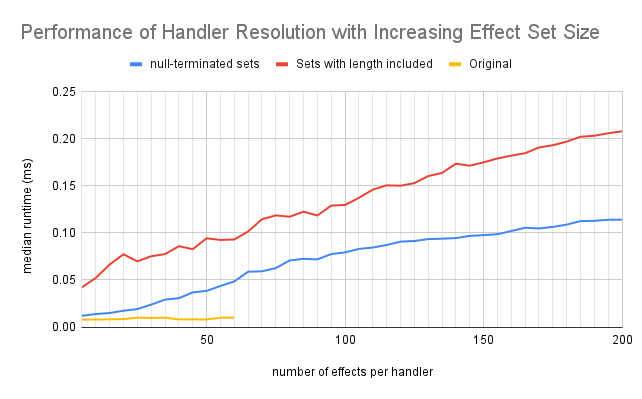
\includegraphics[width=\linewidth]{width_parametrized_performance.png}
    \caption{}
    \label{fig:adjusted}
\end{figure}

A new family of benchmarks, $handler\_stack\_bench$, was written to test the new, more expressive implementation against the original code in the worst possible conditions. A large handler stack with a large number of handled effects on each level is created and the program must find the relevant handler several times, which in both implementations involves checking each level to see if it handles the performed effect. \Cref{fig:adjusted} contains the results of this benchmarking as the number of effects each of the intermediate handlers handles increases.

\begin{figure}[ht]
    \centering
    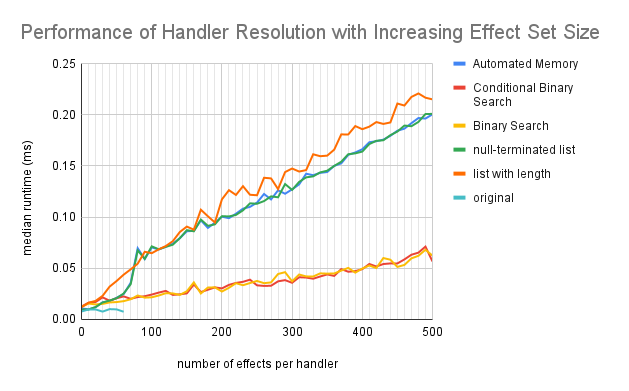
\includegraphics[width=\linewidth]{lines_new.png}
    \caption{}
    \label{fig:parametrized_actual}
\end{figure}

Note that the original \textbf{libseff} implementation is asymptotically faster, as well as being faster for any number of effects tested, but cannot handle any number of effects above 63 (as an effect tag is reserved for the predefined RETURN effect).

With this being the case, it was found that null terminated sets were the faster solution.

\begin{comment}
Specifics: 

\begin{itemize}
    \item $thin$: each intermediate handler handles 1 effect
    \item $mid$: each intermediate handler handles 12 effects
    \item $wide$: each intermediate handler handles 32 effects
    \item $real$: each intermediate handler handles 32 effects, and the effect is performed and then returned from rather than manually searching for the given handler. This is equivalent to $wide$ with an extra effect performance per iteration, along with the overhead that entails, and is a little more realistic.
\end{itemize}

The below graph shows the results:

\todo{Results!!}

This graph shows that the generic benchmarks showed no significant performance difference between versions, while the dedicated microbenchmarks showed a significant slowdown only in the worst case.


Benchmark discussion:





When evaluated against the benchmarks found in the \defcitealias{bench-joint}{joint effect benchmarking library}\citetalias{bench-joint}, it was found that this implementation ran faster than the original implementation on almost all benchmarks, which is an unexpected and slightly confusing, albeit welcome, result.



\begin{itemize}
 \item Created 4 new tests which test the performance with different handler widths
 \item adjusted the iteration parameters for the $ad\_bench$ tests up to get results that don't just depend on startup time
 \item Adjusted the iteration parameters for the $exception\_bench$ tests down to prevent an OOM process kill
 \item Edited all benchmarks to use new syntax given above
 \item Could not run $http\_server\_bench\_$, $prefetching\_lookups\_bench\_$, or $memory\_bench\_$ because of dependency issues
 \item Removed $chameneos\_bench$ from the aggregated benchmarks because it was too small to provide equivalent testing and I don't understand it enough to be comfortable seamlessly changing the iteration size
 \item These results suggest that the faster run-times seen in a previous draft were an artefact of the low iteration counts used, although the consistency probably means something?
 \end{itemize}
 

\begin{figure}[ht]
    \centering
    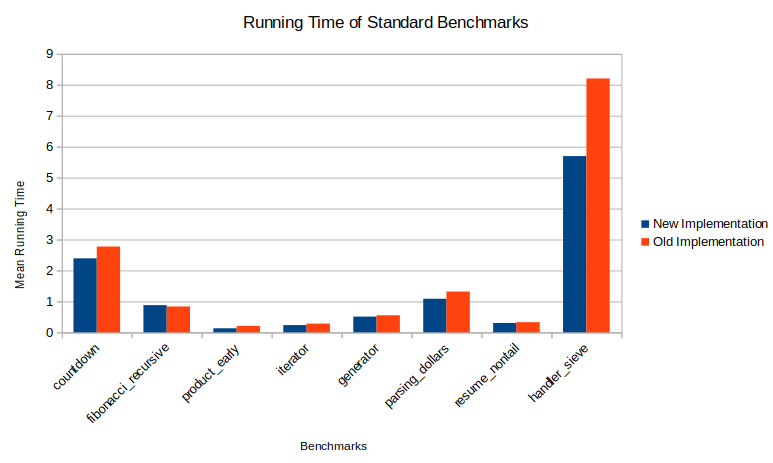
\includegraphics[width=1\linewidth]{bench_tests.PNG}
    \label{fig:benches}
\end{figure}

As we can see from \cref{fig:adjusted}, both implementations perform worse when the handlers iterated through handle a large number of effects, but performance from Implementation 2\cref{impls_here} was clearly superior both when there were very few effects and as a factor to the runtime - i.e. provided both an asymptotic and proportional speedup. The original implementation is faster at all widths that it can support, although tests could not be performed past a certain point because of its limitations.
\end{comment}




\chapter{Conclusion} \label{conc}

%In conclusion, my changes are awesome and should be merged into the main repo thank you sam :)

The \textbf{libseff} library had several limitations, like a requirement that 

% \bibliographystyle{plain}
%\bibliographystyle{plainnat}
%\bibliography{refs}

\addcontentsline{toc}{chapter}{Bibliography}
\printbibliography

\nocite{*}


% You may delete everything from \appendix up to \end{document} if you don't need it.
\appendix

\chapter{Implemented Code} \label{appx}

The implementation of the changes discussed in this document can be found here: 
\url{https://github.com/Pendscraper/libseff_disc}

A full list of the documents cited can be found here:
\url{https://github.com/Pendscraper/libseff_disc_overleaf/tree/main/papers}


\todos
\end{document}
